\documentclass[tikz,border=2mm]{standalone}
\tikzset{global scale/.style={
    	scale=#1,
    	every node/.append style={scale=#1}
  	}
}
\begin{document}
	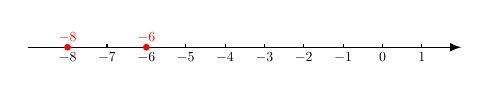
\begin{tikzpicture}[global scale = 0.5]
  		\draw [black, -latex] (-9,0) -- (2,0); 
		\foreach \x in {-8, ..., 1}
			\draw (\x cm,2pt) -- (\x cm,0pt) node[anchor=north] {$\x$};
		% -8, -6, -5, 0.1, -1/4, 0, -4.2, -5.1, 2/3, 3/2, +1/5, 0
		\draw [red, fill=red] (-8, 0) circle(2pt) node [above] {$-8$}; 
		\draw [red, fill=red] (-6, 0) circle(2pt) node [above] {$-6$}; 		
	\end{tikzpicture}    
\end{document}
